\scanpage{116}

$\widetilde{X}^{\substack{*\\*}*\,\unsure{\vcenter{\hbox{\tikz[x=1mm,y=1mm]{\draw[line width=.4pt] (0,0)--(.04,.85);}}}}}$ ; (les trois $*$ signifient qu'on a enlevé \inserted{tous} les points de type $0,1,\infty$, disposés comme suit $\substack{\infty\\0}1$, on définirait de même $\widetilde{X}^{\substack{*\\\cdot}*}$, $\widetilde{X}^{\substack{\unsure{\cdot|*}\\*}*}$, $\widetilde{X}^{\substack{*\\*}\cdot}$, etc. \deleted{Donc} L'intérieur de cette surface à bord, savoir $X\setminus S=X\setminus\{R_\varphi\mid\varphi\in S\}$, est notée $X^{\substack{*\\*}*}$, on définit de $=$ $X^{\substack{*\\\cdot}*}$ etc. Les points $R_r^{ij}$ et les chemins précédents seront regardés, le plus commodément, comme points et chemins, (parfaitement canoniques, pas seulement des classes d'homotopie !) dans $\widetilde{X}^{\substack{*\\*}*}$. On notera que les $R_\varphi$ $(\varphi\in S)$ ne \uline{sont pas} dans $\widetilde{X}^{\substack{*\ *\\*}}$
\tikz[baseline=-.35ex]{
  \draw[line width=.4pt] (0,0)--(.55,.025);
  \node[inner sep=0pt] at (.08,-.18) {$\unsure{\vcenter{\hbox{\tikz[x=1mm,y=1mm,line width=.45pt]{
    \draw (.12,.72) .. controls (-.1,.54) and (.03,.14) .. (.38,.13)
      .. controls (.68,.11) and (.7,.48) .. (.45,.58)
      .. controls (.28,.64) and (.11,.46) .. (.2,.3);
    \draw (.4,.61)--(.77,.18)--(.6,-.03);
  }}}}$};
}
mais dans l'application $C^\infty$ (\unsure{et $=$|$\ne$} analytique réelle) canonique
\diagram{
$(11)\qquad$
\begin{tikzcd}[ampersand replacement=\&]
\widetilde{X}^{\substack{*\\*}*} \arrow[r] \& X
\end{tikzcd}
}
Le point $R_r^{ij}$ va sur $R_r^i=R_\varphi$, où $\varphi$ est le \deleted{point} \inserted{sommet} de type $i$ de $r$.

On a, dans $\Pi_1 X^{\substack{*\\*}*}$, la relation
\reversemarginpar
\margin{\vspace*{1.8\baselineskip}
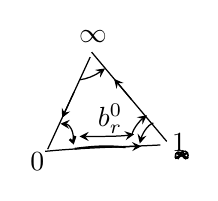
\begin{tikzpicture}[x=.9cm,y=.9cm,>=stealth,line width=.45pt]
  % Three separately drawn contours: small pen gaps at the apex and at 1.
  \draw (.02,.02)--(.62,1.32);
  \draw (.64,1.39)--(1.7,.13);
  \draw (-.015,-.01) .. controls (.54,.045) and (1.17,.055) .. (1.61,.08);
  \draw[line width=.7pt] (.4,.026) .. controls (.77,.075) and (.92,.063) .. (1.12,.048);
  \draw[->] (.392,.826)--(.224,.462);
  \draw[->] (1.2,.724)--(.958,1.012);
  \draw[->] (.91,.049)--(1.34,.061);
  % The three corner arcs, with the dense lower endpoint at 0 retained as ink.
  \draw[->] (.472,1.0) .. controls (.57,1.01) and (.68,1.055) .. (.83,1.16);
  \draw[<-] (.2,.38) .. controls (.34,.37) and (.41,.22) .. (.37,.13);
  \draw[line width=.85pt] (.33,.16)--(.38,.115)--(.41,.205);
  \draw[->] (1.51,.39) .. controls (1.42,.36) and (1.35,.22) .. (1.32,.1);
  % Opposed heads on the inner horizontal part, followed by the rising segment.
  \draw[<->] (.47,.2) .. controls (.8,.2) and (1.04,.2) .. (1.24,.23);
  \draw[->] (1.21,.23) .. controls (1.23,.32) and (1.33,.43) .. (1.42,.5);
  \node[below left,inner sep=1pt] at (.02,.02) {$0$};
  \node[right,inner sep=1pt] at (1.73,.12) {$1$};
  \node[above,inner sep=1pt] at (.66,1.48) {$\infty$};
  \node at (.9,.45) {$b_r^0$};
  % Dense overwritten or cancelled label below the live 1: identity/state doubtful.
  \node[inner sep=0pt] at (1.91,-.06) {$\unsure{\vcenter{\hbox{\tikz[x=1mm,y=1mm,line width=.55pt]{
    \draw (0,.35) .. controls (-.08,1.03) and (.64,1.25) .. (.91,.59)
      .. controls (1.08,.02) and (1.57,.01) .. (1.63,.55)
      .. controls (1.69,1.12) and (.91,1.35) .. (.61,.72)
      .. controls (.38,.26) and (.15,.02) .. (0,.35);
    \draw[line width=.8pt] (-.04,.21)--(1.52,.85);
    \draw[line width=.7pt] (.12,.85)--(1.66,.2);
    \draw (.31,.09)--(.94,1.05)--(1.38,.08);
  }}}}$};
\end{tikzpicture}}
\normalmarginpar
\[
(12)\qquad
\boxed{
\underbrace{(\lambda_r^0)^{-1}a_r^1}_{\underset{=}{\text{def}}\ b_r^\infty}
\underbrace{(\lambda_r^\infty)^{-1}a_r^0}_{b_r^1}
\underbrace{(\lambda_r^1)^{-1}a_r^\infty}_{b_r^0}=1
}
\qquad\text{lacet en }R_r^{1\infty}
\]
Les sommets $R_r^{ij}$, les flèches $\lambda_r^i$ et $a_r^i$, et les relations $(10)$ $(17)$, forment une présentation du groupoïde $\Pi_1(\widetilde{X}^{\substack{*\\*}*},\unsure{\{|(}R_r^{i,j}))$.

\mspage{115}
